\documentclass[border=0.2cm]{standalone}
 
% Pie chart drawing library 
\usepackage{pgf-pie}  
 
\begin{document}
 


\begin{minipage}{0.23\linewidth}
Blabla
Blabla
Blabla
Blabla
Blabla
Blabla
Blabla
Blabla
Blabla
Blabla
Blabla
Blabla
Blabla
Blabla
\end{minipage}
\hfill
\begin{minipage}{0.75\linewidth}
\begin{center}
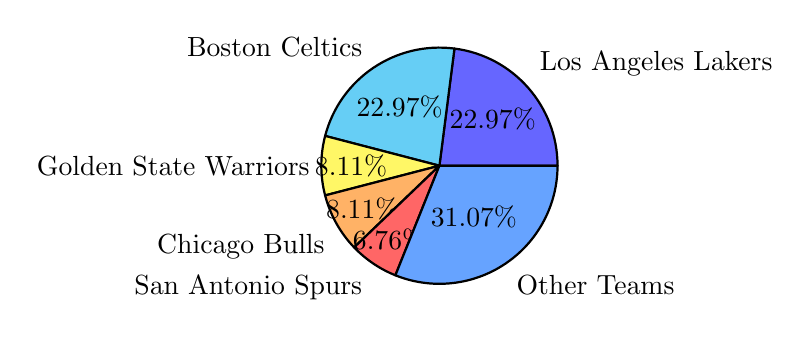
\begin{tikzpicture}[scale=0.5] 
\pie{22.97/Los Angeles Lakers,
    22.97/Boston Celtics,
    8.11/Golden State Warriors,
    8.11/Chicago Bulls,
    6.76/San Antonio Spurs,
    31.07/Other Teams}
 
\end{tikzpicture}
\end{center}
\end{minipage}

 
\end{document}

Un blog intéressant pour les figures :
https://latexdraw.com/how-to-plot-a-pie-chart-in-latex/

Document sur CTAN :
https://ctan.org/pkg/pgf-pie